\section{Radio Definida por Software}

%\subsection{SDR, surgimiento y utilizacion actual}

\begin{frame}{Radio Definida por Software}
\begin{block}{SDR (Software Defined Radio)}
	\begin{itemize}
		%\subsection{ISDB-T (International Standard for Digital Broadcasting - Terrestrial)}	
		\item {	¿Qué es? }
		\item { ¿Qué ventajas tiene? }
		\item { La utilización de SDR en gr-isdbt-Tx}
	\end{itemize}
\end{block}
\end{frame}

%\subsection{GNU Radio}
\begin{frame}
\frametitle{Radio Definida por Software}
\begin{columns}
	\column{0.5\textwidth}
	\begin{itemize}	
		\item { Software de código abierto para SDR}
		\item {	Flowgraphs y Bloques }
		\item { La creación de bloques personalizados }
	\end{itemize}
	\column{0.5\textwidth}
	\begin{figure}
		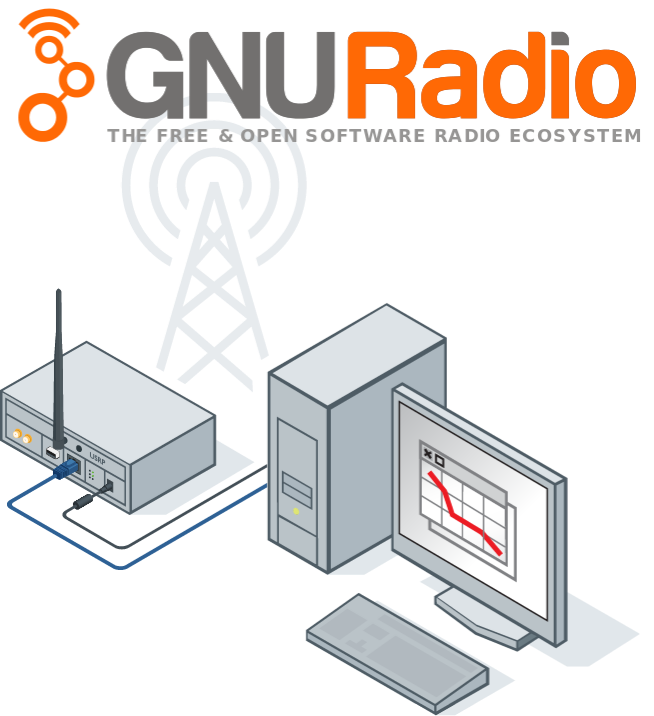
\includegraphics[scale=0.25]{sdr}
		\caption{GNU Radio}
	\end{figure}
\end{columns}
\end{frame}

\begin{frame}{GNU Radio}
	\begin{figure}
	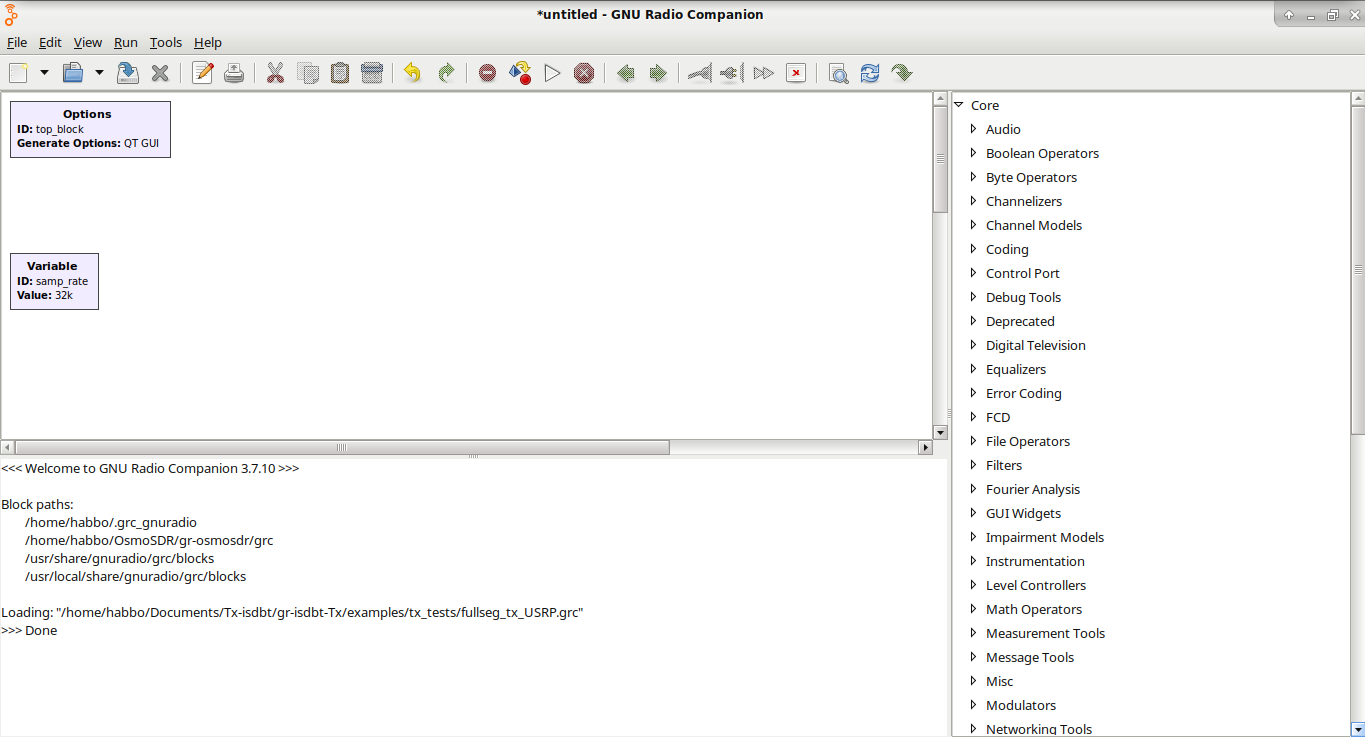
\includegraphics[scale=0.22]{grc}
	\caption{GNU Radio framework}
	\end{figure}
\end{frame}

%\subsection{El hardware utilizado}
\begin{frame}
\frametitle{El hardware utilizado}
\begin{columns}
	\column{0.5\textwidth}
		\begin{itemize}	
			\item {Ettus Research B100}
		\end{itemize}
		\begin{figure}
		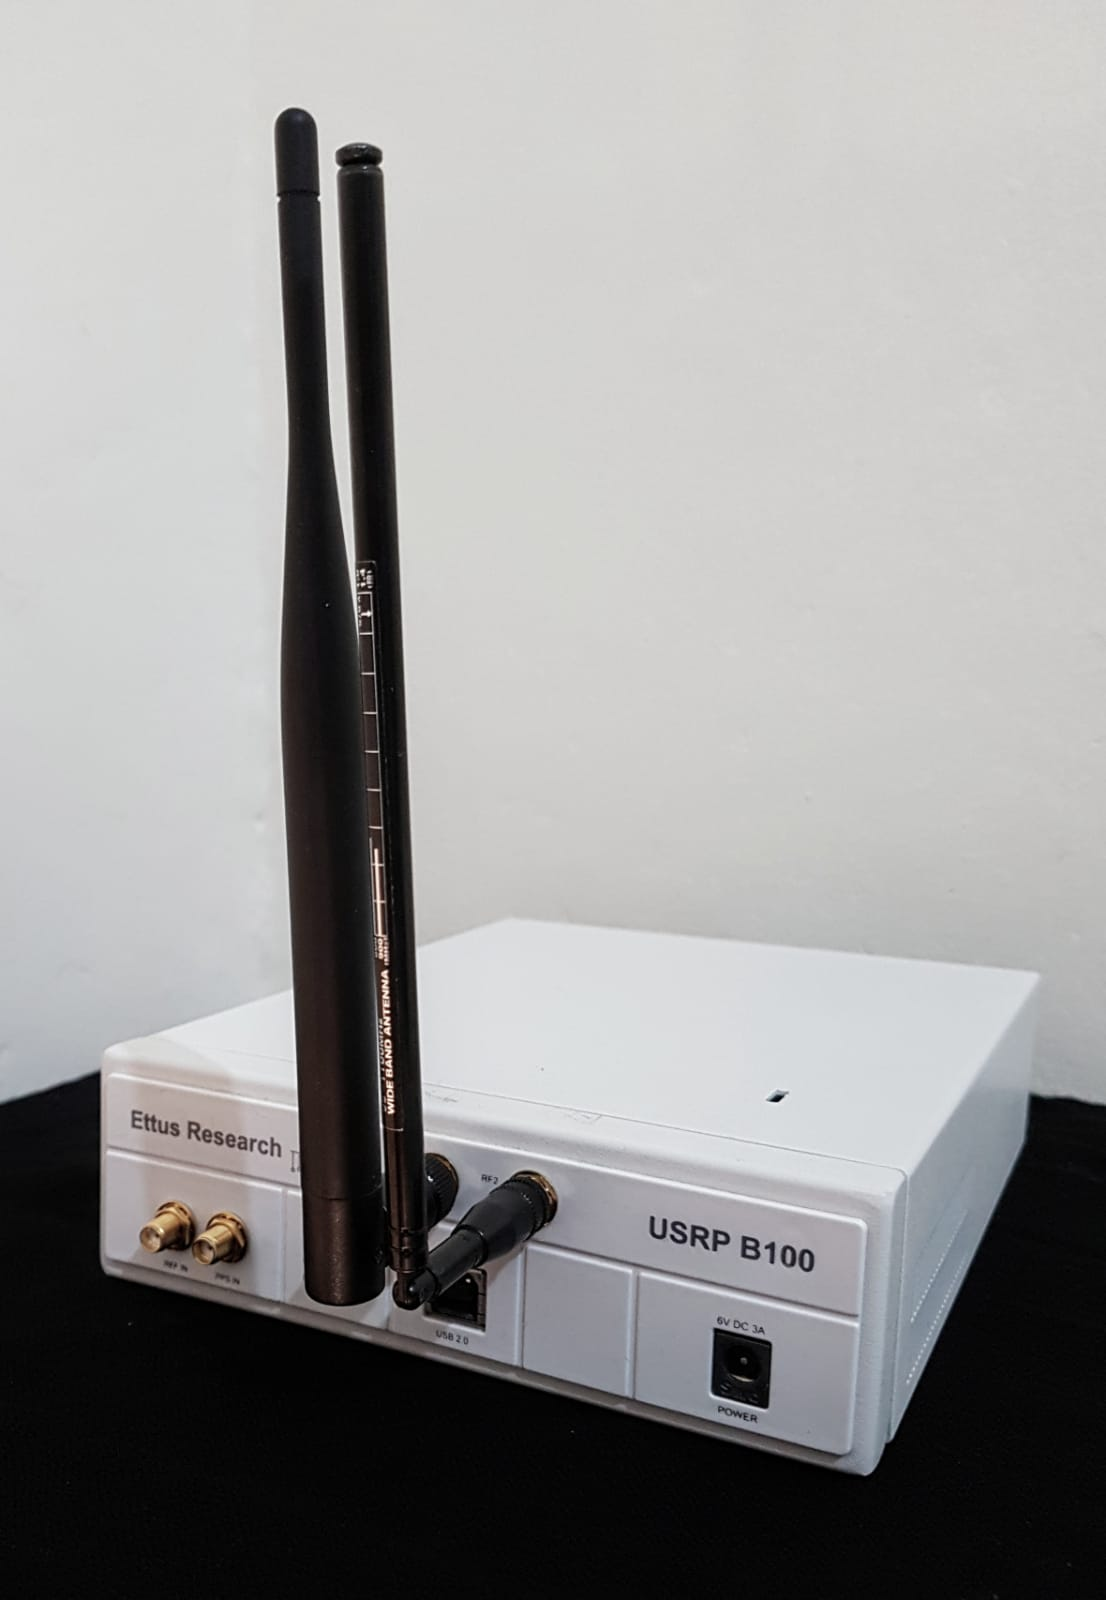
\includegraphics[scale=0.10]{usrp_foto}
		\caption{USRP B100}
		\end{figure}
	\column{0.5\textwidth}
		\begin{itemize}	
			\item { Antenas de uso múltiple}
		\end{itemize}
		\begin{figure}
			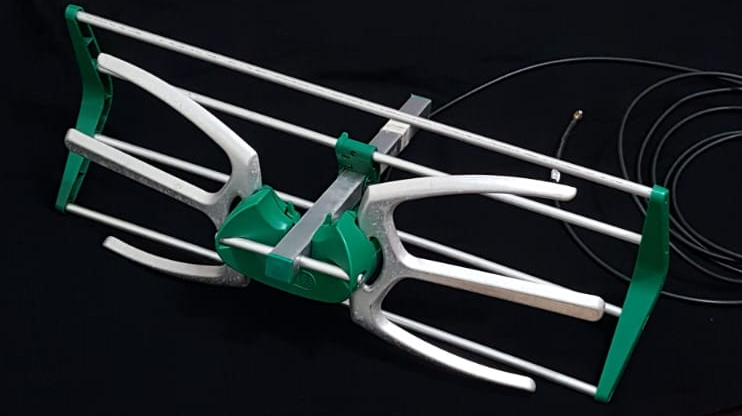
\includegraphics[scale=0.20]{antena}
			\caption{Antena para la banda de TV}
		\end{figure}
\end{columns}
\end{frame}